\documentclass[12pt]{article}
\usepackage[margin=2cm, top = 2.5 cm]{geometry}
\usepackage{graphicx,tikz,tikz-network,tkz-euclide}
\usepackage{amsfonts,amsmath,amssymb}
\usepackage{tasks}
\usepackage{enumitem}
\usepackage{fancyhdr}
\usepackage{ifthen}
\usepackage{xparse}
\usepackage{tabularx}
\usepackage{marginnote}
\usepackage{cancel}
\usepackage{tcolorbox}
\usepackage{adjustbox}
\usetikzlibrary{positioning}
\definecolor{processblue}{cmyk}{0.96,0,0,0}
\definecolor{midnightblue}{HTML}{006699}

% for synthetic division in problem A3
\newcommand{\synthdivbox}[1]{%
    \makebox[0pt][l]{\rule[-.4em]{\widthof{#1}+.5em}{.4pt}}% 
    \makebox[\widthof{#1}+.5em][c]{#1}\vrule%
    }

%\title{Math Club Seventh Week}
%\date{November 2024}

\fancyhead[L]{Math Club W8\ifthenelse{\boolean{showsolutions}}{ (Solutions)}{}}
\fancyhead[R]{Nov 11, 2024}

\parindent 0pt
\marginparsep 3pt

\newcounter{problem}
\setcounter{problem}{0} % Initialize the counter at 0
\newcounter{sectionB}
\setcounter{sectionB}{0}

%\problem[source][difficulty]{problem text}
\NewDocumentCommand{\problem}{O{} o m}{
    \stepcounter{problem}%
    \noindent%
    \ifthenelse{\equal{\theproblem}{1}}{}{\\[1mm]}%
    % Determine difficulty level exclamation marks
    \IfNoValueTF{#2}{}{\reversemarginpar\marginnote{\color{red}\hfill\textbf{#2}}\reversemarginpar}%
    \textbf{Problem $\mathbf{A\theproblem}$:}%
    \ifthenelse{\equal{#1}{}}{}{ (#1)}% Only include parentheses if (#1) if available
    \\[1mm]#3\\[1.5mm]
    }

\NewDocumentCommand{\problemB}{O{} o m}{
    \stepcounter{sectionB}%
    \noindent%
    \ifthenelse{\equal{\thesectionB}{1}}{}{\\[1mm]}%
    % Determine difficulty level exclamation marks
    \IfNoValueTF{#2}{}{\reversemarginpar\marginnote{\color{red}\hfill\textbf{#2}}\reversemarginpar}%
    \textbf{Problem $\mathbf{B\thesectionB}$:}%
    \ifthenelse{\equal{#1}{}}{}{ (#1)}% Only include parentheses if (#1) if available
    \\[1mm]#3\\[1.5mm]
    }

\newcommand{\multChoice}[5]{%
{\centering
\begin{tabular}{l @{\hskip 1.5cm} l @{\hskip 1.5cm} l @{\hskip 1.5cm} l @{\hskip 1.5cm} l}%
    A. #1 & B. #2 & C. #3 & D. #4 & E. #5
\end{tabular} \par}
}

\NewDocumentCommand{\multOpt}{O{3} m o o o o o o o}{%
    \ExplSyntaxOn%
    \renewcommand{\arraystretch}{1}% Adjust spacing between rows if needed
    \begin{tabularx}{\textwidth}{@{}*{#1}{>{\centering\arraybackslash}X}@{}}%
        A. #2%
        \IfValueT{#3}{ & B. #3}%
        \IfValueT{#4}{ & C. #4}%
        \IfValueT{#5}{ & D. #5}%
        \IfValueT{#6}{ & E. #6}%
        \IfValueT{#7}{ & F. #7}%
        \IfValueT{#8}{ & G. #8}%
        \IfValueT{#9}{ & H. #9}%
  \end{tabularx}%
  \ExplSyntaxOff%
}%

\NewDocumentCommand{\myFloor}{o m}{%
  \ensuremath{%
  \left\lfloor%
  \IfValueTF{#1}{%
    \frac{#2}{#1}%
  }{%
    #2%
  }
  \right\rfloor%
  }
}

\newboolean{showsolutions}
\setboolean{showsolutions}{false}
\newcommand{\solution}[2][]{%
    \ifthenelse{\boolean{showsolutions}}{%
    \vspace{1em}\noindent\textbf{Solution:} #1%
    \\[0.4mm]#2
    }{}%
}

\setlength{\baselineskip}{5\baselineskip}
\setlength{\parskip}{5pt}

\newcommand{\myVertex}[3]{
    \Vertex[x=#1,y=#2,size=0.5,label=$#3$,position=90,fontscale=2,style={color=red}]{#3}
}
\newcommand{\simpleVertex}[3]{
    \Vertex[x=#1,y=#2,size=0.5,position=180,fontscale=2,style={color=red}]{#3}
}
\newcommand{\invisibleVertex}[3]{
    \Vertex[x=#1,y=#2,size=0.5,opacity =0,position=180,fontscale=2,style={color=white}]{#3}
}

\begin{document}
%SHOW OR HIDE SOLUTIONS
\setboolean{showsolutions}{true}

\sloppy
\thispagestyle{fancy}

\section*{AMATYC problems}
\vspace{-6mm}
%\hbox to \textwidth{

\begin{problem}[C][2][AMATYC Spring 2017/5]
   % Discrete ^ Student Math League
\begin{minipage}[b][][b]{0.75\textwidth}\vspace{0pt}%
In the grid (made up of \(1 \times 1\) squares) on the right, which of the squares \(A\), \(B\), \(C\), \(D\), or \(E\), when shaded, will allow the unshaded squares to be covered by exactly 14 dominos (\(1 \times 2\) rectangles) with no overlaps or gaps?
\end{minipage}\hfill%
\begin{minipage}[b][][b]{0.2\textwidth}%
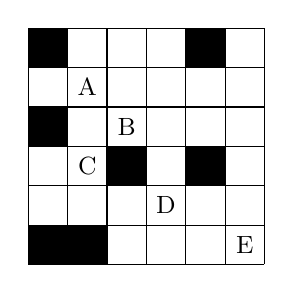
\begin{tikzpicture}[scale=0.5]
% Draw the 6x6 grid
\draw (0,0) grid (6,6);
% Fill black squares
\fill[black] (0,5) rectangle (1,6);
\fill[black] (4,5) rectangle (5,6);
\fill[black] (0,3) rectangle (1,4);
\fill[black] (2,2) rectangle (3,3);
\fill[black] (4,2) rectangle (5,3);
\fill[black] (0,0) rectangle (1,1);
\fill[black] (1,0) rectangle (2,1);
% Add letters
\node[font=\small] at (1.5,4.5) {A};
\node[font=\small] at (2.5,3.5) {B};
\node[font=\small] at (1.5,2.5) {C};
\node[font=\small] at (3.5,1.5) {D};
\node[font=\small] at (5.5,0.5) {E};
\end{tikzpicture}\vspace{4.5mm}
\end{minipage}\vspace{-5mm}
\end{problem}


\begin{solution}[D]
   Consider where in the grid the dominos are forced to be placed and oriented in a certain way to avoid leaving a gap. At first, there are two such places (filled in with red dominos below).\par\vspace{-5pt}
\begin{minipage}[t][][t]{0.3\linewidth}\vspace{0pt}%
Once these are filled in, they force additional dominos to be placed, ruling out more and more letters until only $D$ and $E$ remain.
\end{minipage}\hspace{0.02\linewidth}\hfill%
\begin{minipage}[t][][t]{0.15\linewidth}\vspace{0pt}%
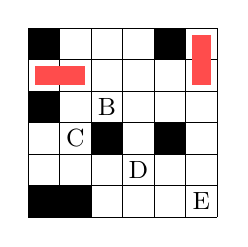
\begin{tikzpicture}[scale=0.4]
% Draw the 6x6 grid
\draw (0,0) grid (6,6);
% Fill black squares
\fill[black] (0,5) rectangle (1,6);
\fill[black] (4,5) rectangle (5,6);
\fill[black] (0,3) rectangle (1,4);
\fill[black] (2,2) rectangle (3,3);
\fill[black] (4,2) rectangle (5,3);
\fill[black] (0,0) rectangle (1,1);
\fill[black] (1,0) rectangle (2,1);
\fill[red!70] (0.2,4.2) rectangle (1.8,4.8); %horizontal
\fill[red!70] (5.2,4.2) rectangle (5.8,5.8); %vertical
% Add letters
\node[font=\small] at (2.5,3.5) {B};
\node[font=\small] at (1.5,2.5) {C};
\node[font=\small] at (3.5,1.5) {D};
\node[font=\small] at (5.5,0.5) {E};
\end{tikzpicture}
\end{minipage}\hfill%
%
\begin{minipage}[t][][t]{0.15\linewidth}\vspace{0pt}%
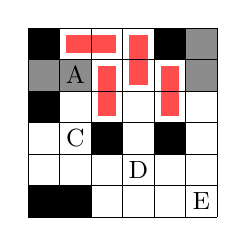
\begin{tikzpicture}[scale=0.4]
% Fill black squares
\fill[black] (0,5) rectangle (1,6);
\fill[black] (4,5) rectangle (5,6);
\fill[black] (0,3) rectangle (1,4);
\fill[black] (2,2) rectangle (3,3);
\fill[black] (4,2) rectangle (5,3);
\fill[black] (0,0) rectangle (1,1);
\fill[black] (1,0) rectangle (2,1);
\fill[black!45] (0,4) rectangle (2,5);
\fill[black!45] (5,4) rectangle (6,6);
\fill[red!70] (1.2,5.2) rectangle (2.8,5.8);
\fill[red!70] (3.2,4.2) rectangle (3.8,5.8); 
\fill[red!70] (2.2,3.2) rectangle (2.8,4.8);
\fill[red!70] (4.2,3.2) rectangle (4.8,4.8);
% Draw the 6x6 grid
\draw (0,0) grid (6,6);
% Add letters
\node[font=\small] at (1.5,4.5) {A};
\node[font=\small] at (1.5,2.5) {C};
\node[font=\small] at (3.5,1.5) {D};
\node[font=\small] at (5.5,0.5) {E};
\end{tikzpicture}
\end{minipage}\hfill%
%
\begin{minipage}[t][][t]{0.15\linewidth}\vspace{0pt}%
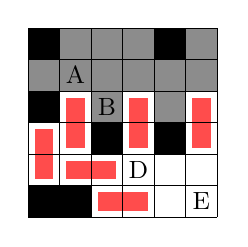
\begin{tikzpicture}[scale=0.4]
%
\fill[black] (0,5) rectangle (1,6);
\fill[black] (4,5) rectangle (5,6);
\fill[black] (0,3) rectangle (1,4);
\fill[black] (2,2) rectangle (3,3);
\fill[black] (4,2) rectangle (5,3);
\fill[black] (0,0) rectangle (1,1);
\fill[black] (1,0) rectangle (2,1);
\fill[black!45] (0,4) rectangle (2,5);
\fill[black!45] (5,4) rectangle (6,6);
\fill[black!45] (1,5) rectangle (3,6);
\fill[black!45] (3,4) rectangle (4,6);
\fill[black!45] (2,3) rectangle (3,5);
\fill[black!45] (4,3) rectangle (5,5);
\fill[red!70] (0.2,1.2) rectangle (0.8,2.8);
\fill[red!70] (1.2,2.2) rectangle (1.8,3.8);
\fill[red!70] (3.2,2.2) rectangle (3.8,3.8);
\fill[red!70] (5.2,2.2) rectangle (5.8,3.8);
\fill[red!70] (1.2,1.2) rectangle (2.8,1.8); 
\fill[red!70] (2.2,0.2) rectangle (3.8,0.8); 
%
\draw (0,0) grid (6,6);
%
\node[font=\small] at (1.5,4.5) {A};
\node[font=\small] at (2.5,3.5) {B};
%\node[font=\small] at (1.5,2.5) {C};
\node[font=\small] at (3.5,1.5) {D};
\node[font=\small] at (5.5,0.5) {E};
\end{tikzpicture}
\end{minipage}\hfill%
%
\begin{minipage}[t][][t]{0.15\linewidth}\vspace{0pt}%
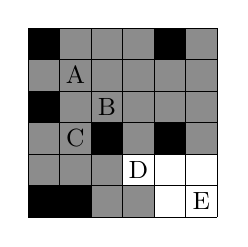
\begin{tikzpicture}[scale=0.4]
%
\fill[black] (0,5) rectangle (1,6);
\fill[black] (4,5) rectangle (5,6);
\fill[black] (0,3) rectangle (1,4);
\fill[black] (2,2) rectangle (3,3);
\fill[black] (4,2) rectangle (5,3);
\fill[black] (0,0) rectangle (1,1);
\fill[black] (1,0) rectangle (2,1);
\fill[black!45] (0,4) rectangle (2,5);
\fill[black!45] (5,4) rectangle (6,6);
\fill[black!45] (1,5) rectangle (3,6);
\fill[black!45] (3,4) rectangle (4,6);
\fill[black!45] (2,3) rectangle (3,5);
\fill[black!45] (4,3) rectangle (5,5);
\fill[black!45] (0,1) rectangle (1,3);
\fill[black!45] (1,2) rectangle (2,4);
\fill[black!45] (3,2) rectangle (4,4);
\fill[black!45] (5,2) rectangle (6,4);
\fill[black!45] (1,1) rectangle (3,2);
\fill[black!45] (2,0) rectangle (4,1);
%
\draw (0,0) grid (6,6);
%
\node[font=\small] at (1.5,4.5) {A};
\node[font=\small] at (2.5,3.5) {B};
\node[font=\small] at (1.5,2.5) {C};
\node[font=\small] at (3.5,1.5) {D};
\node[font=\small] at (5.5,0.5) {E};
\end{tikzpicture}
\end{minipage}\hspace{0pt}\\[-5pt]
\par
\begin{minipage}[t][][t]{0.48\linewidth}\vspace{0pt}
You're now left with two possible layouts, but they both result in $E$ being covered up with a domino and $D$ being the only unoccupied square remaining. Thus, \fbox{D} should be shaded.
\end{minipage}\hspace{6pt}\hfill%
\begin{minipage}[t][][t]{0.15\linewidth}\vspace{0pt}%
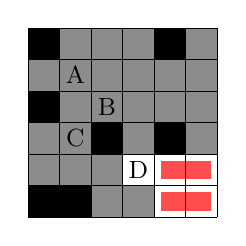
\begin{tikzpicture}[scale=0.4]
%
\fill[black] (0,5) rectangle (1,6);
\fill[black] (4,5) rectangle (5,6);
\fill[black] (0,3) rectangle (1,4);
\fill[black] (2,2) rectangle (3,3);
\fill[black] (4,2) rectangle (5,3);
\fill[black] (0,0) rectangle (1,1);
\fill[black] (1,0) rectangle (2,1);
\fill[black!45] (0,4) rectangle (2,5);
\fill[black!45] (5,4) rectangle (6,6);
\fill[black!45] (1,5) rectangle (3,6);
\fill[black!45] (3,4) rectangle (4,6);
\fill[black!45] (2,3) rectangle (3,5);
\fill[black!45] (4,3) rectangle (5,5);
\fill[black!45] (0,1) rectangle (1,3);
\fill[black!45] (1,2) rectangle (2,4);
\fill[black!45] (3,2) rectangle (4,4);
\fill[black!45] (5,2) rectangle (6,4);
\fill[black!45] (1,1) rectangle (3,2);
\fill[black!45] (2,0) rectangle (4,1);
\fill[red!70] (4.2,1.2) rectangle (5.8,1.8);
\fill[red!70] (4.2,0.2) rectangle (5.8,0.8);
%
\draw (0,0) grid (6,6);
%
\node[font=\small] at (1.5,4.5) {A};
\node[font=\small] at (2.5,3.5) {B};
\node[font=\small] at (1.5,2.5) {C};
\node[font=\small] at (3.5,1.5) {D};
\end{tikzpicture}
\end{minipage}\hfill%
%
\begin{minipage}[t][][t]{0.15\linewidth}\vspace{0pt}%
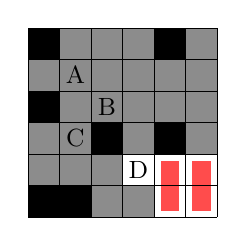
\begin{tikzpicture}[scale=0.4]
%
\fill[black] (0,5) rectangle (1,6);
\fill[black] (4,5) rectangle (5,6);
\fill[black] (0,3) rectangle (1,4);
\fill[black] (2,2) rectangle (3,3);
\fill[black] (4,2) rectangle (5,3);
\fill[black] (0,0) rectangle (1,1);
\fill[black] (1,0) rectangle (2,1);
\fill[black!45] (0,4) rectangle (2,5);
\fill[black!45] (5,4) rectangle (6,6);
\fill[black!45] (1,5) rectangle (3,6);
\fill[black!45] (3,4) rectangle (4,6);
\fill[black!45] (2,3) rectangle (3,5);
\fill[black!45] (4,3) rectangle (5,5);
\fill[black!45] (0,1) rectangle (1,3);
\fill[black!45] (1,2) rectangle (2,4);
\fill[black!45] (3,2) rectangle (4,4);
\fill[black!45] (5,2) rectangle (6,4);
\fill[black!45] (1,1) rectangle (3,2);
\fill[black!45] (2,0) rectangle (4,1);
\fill[red!70] (4.2,0.2) rectangle (4.8,1.8);
\fill[red!70] (5.2,0.2) rectangle (5.8,1.8);
%
\draw (0,0) grid (6,6);
%
\node[font=\small] at (1.5,4.5) {A};
\node[font=\small] at (2.5,3.5) {B};
\node[font=\small] at (1.5,2.5) {C};
\node[font=\small] at (3.5,1.5) {D};
\end{tikzpicture}
\end{minipage}\hfill%
%
\begin{minipage}[t][][t]{0.15\linewidth}\vspace{0pt}%
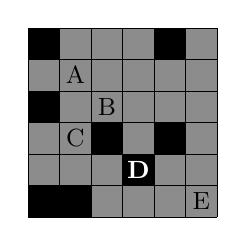
\begin{tikzpicture}[scale=0.4]
%squares
\fill[black] (0,5) rectangle (1,6);
\fill[black] (4,5) rectangle (5,6);
\fill[black] (0,3) rectangle (1,4);
\fill[black] (2,2) rectangle (3,3);
\fill[black] (4,2) rectangle (5,3);
\fill[black] (0,0) rectangle (1,1);
\fill[black] (1,0) rectangle (2,1);
\fill[black] (3,1) rectangle (4,2);
\fill[black!45] (0,4) rectangle (2,5);
\fill[black!45] (5,4) rectangle (6,6);
\fill[black!45] (1,5) rectangle (3,6);
\fill[black!45] (3,4) rectangle (4,6);
\fill[black!45] (2,3) rectangle (3,5);
\fill[black!45] (4,3) rectangle (5,5);
\fill[black!45] (0,1) rectangle (1,3);
\fill[black!45] (1,2) rectangle (2,4);
\fill[black!45] (3,2) rectangle (4,4);
\fill[black!45] (5,2) rectangle (6,4);
\fill[black!45] (1,1) rectangle (3,2);
\fill[black!45] (2,0) rectangle (4,1);
\fill[black!45] (4,0) rectangle (6,2);
%
\draw (0,0) grid (6,6);
%
\node[font=\small] at (1.5,4.5) {A};
\node[font=\small] at (2.5,3.5) {B};
\node[font=\small] at (1.5,2.5) {C};
\node[font=\small, white!70] at (3.5,1.5) {\textbf{D}};
\node[font=\small] at (5.5,0.5) {E};
\end{tikzpicture}
\end{minipage}\hspace{0pt}\par

\end{solution}

\begin{problem}[A][2][AMATYC Fall 2012/12]
   % Inequalities ^ Algebra ^ Student Math League
   If \( \log_2 x \) and \( \log_2 y \) are distinct positive integers and \( \log_x 2 + \log_y 2 = 0.5 \), then \( xy = \)
\end{problem}
\multOpt[5]{64}[128][256][512][1024]
\begin{solution}[D]
   Since both logarithms are positive integers, we must have $m,n \in \mathbb{Z}^+$ such that $x=2^m$ and $y=2^n$. But before, remember that 
    $\log_ab \cdot \log_ba = \log_aa=1$, so $\log_ab=1/\log_ba$
    \\From it the equation becomes 
    \begin{align}
        \frac{1}{m} + \frac{1}{n} = \frac{1}{2}
    \end{align}
    Assume without loss of generality that $m>n$, since the equation is symmetric, we want to find a plausible range for $n$, for example we know that $n \notin \{1,2\}$ since the Left-Hand Side of (1) would become bigger than $1/2$:
    \begin{align*}
        &\text{if $2\geq n$:  } \frac{1}{m}+\frac{1}{n} > \frac{1}{n} \geq \frac{1}{2} \rightarrow \hspace{3pt} \leftarrow \\
        &\text{if $n\geq 4$:  } \frac{1}{m}+\frac{1}{n} \leq \frac{1}{4} + \frac{1}{5} < \frac{1}{2} \rightarrow \hspace{3pt} \leftarrow \\
    \end{align*}
    Both cases are contradictions , so we must have $4>n>2$, the only integer in that range is $n=3$, which further implies $m=6$, therefore $xy$=$2^m \cdot 2^n = 2^9=512$
\end{solution}

\begin{problem}[C][1][AMATYC Spring 2017/16]
   % Floor Function ^ Inclusion - Exlusion Principle ^ Student Math League
   How many positive integers less than 1000 are divisible by exactly one of 7 or 11?
\end{problem}
\multOpt[5]{196}[208][220][232][244]
\begin{solution}[C]
    Note that for any $a,n \in \mathbb{Z}^+$, there are $r=\lfloor \frac{n}{a} \rfloor$ integers divisible by $a$ in $[1,n]$ , namely $\{a,2a,\ldots,ra\}$. For us to have integers divisible by exactly one of 7 and 11, we need to get the $r$ for both and subtract the numbers that are divisible by both at the same time, that is, those divisible by 77.
    $$ \myFloor[7]{1000}+\myFloor[11]{1000}-\myFloor[77]{1000} = 220$$
\end{solution}

\begin{problem}[C][1][AMATYC Spring 2022/2]
   % Discrete ^ Student Math League
   \begin{minipage}[b][][b]{0.75\linewidth}\vspace{0pt}%   
      A child wishes to color each of the six states on a map as shown. What is the minimum number of different color crayons she will need to use if each state must be a different color than all states to which it is adjacent?    
      \end{minipage}\hfill%
      \begin{minipage}[b][][b]{0.2\linewidth}%
        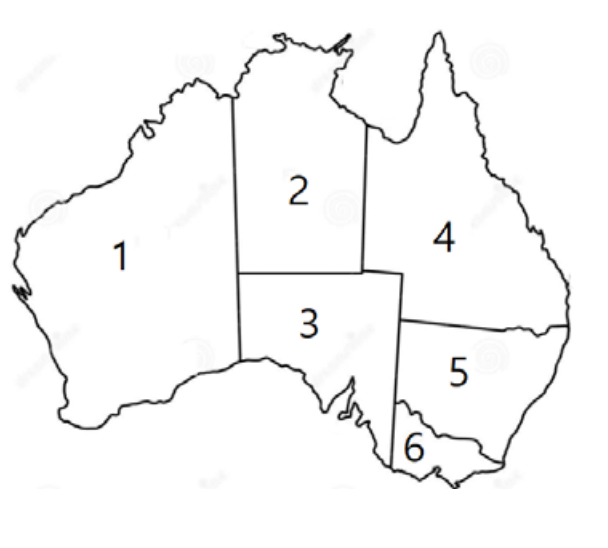
\includegraphics[width=0.9\textwidth]{map.png}
      \vspace{4.5mm}
      \end{minipage}\vspace{-5mm}
\end{problem}
\multOpt[5]{2}[3][4][5][6]

\begin{solution}[B]
   Call $v_i$ to the $i$-th state $(1\leq i \leq 6)$, note that $v_3$ is connected to every other state and color it yellow, now we can't have any other state to be yellow, so we need a new color, take $v_2$ and color it blue, this implies that $v_1$ and $v_4$ can't be neither blue nor yellow, so we need at least three colors, a possible setting is drawn on the right
\end{solution}

\begin{solution}[B]
\begin{minipage}[b][][b]{0.75\linewidth}\vspace{0pt}%
    Call $v_i$ to the $i$-th state $(1\leq i \leq 6)$, note that $v_3$ is connected to every other state and color it yellow, now we can't have any other state to be yellow, so we need a new color, take $v_2$ and color it blue, this implies that $v_1$ and $v_4$ can't be neither blue nor yellow, so we need at least three colors, a possible setting is drawn on the right
\end{minipage}\hfill%
\begin{minipage}[b][][b]{0.2\linewidth}%
  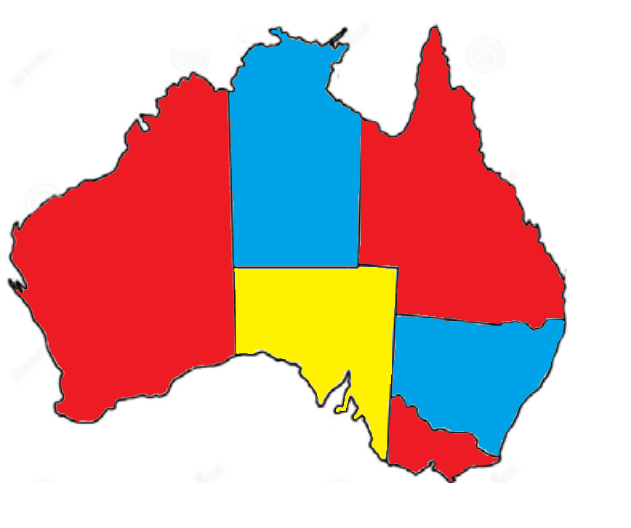
\includegraphics[width=0.9\textwidth]{painted_map.png}
\vspace{3mm}
\end{minipage}
\end{solution}
\vspace{-5mm}

\begin{problem}[C][3][AMATYC Spring 2010/18]
   % Counting ^ MOD ^ Probability ^ Student Math League
   A palindrome is a positive integer like 11, 313, and 5445 which reads the same left to right and right to left. If a number is chosen at random from all four-digit palindromes, find the probability that it is divisible by 7.
\end{problem}
\multOpt[5]{1/7}[1/6][2/11][1/5][2/7]

\begin{solution}[D]
    A four-digit palindrome is of the form $ABBA$ where $A,B$ are digits and $A\neq0$. Let's call $n$ our palindrome so we have
    \begin{align*}
        n &= 1000A+100B+10B+A\\ 
        &= 1001A+110B\\
        \Rightarrow\ n &\equiv 5B \pmod7
    \end{align*}
    So $7\mid n$ only when $B=0$ or $B=7$ which is 2 out of 10 possible values. Thus, the probability of being divisible by 7 is $\boxed{1/5}$. 
\end{solution}

\begin{problem}[A][2][AMATYC Spring 2016/12]
   % Algebra ^ Student Math League
   What is the reminder when $x^{2000}-2x^{15}+2$ is divided by $x^2-1$?
   \multOpt[5]{$3-2x$}[$2x-3$][$2x+3$][$-2x-3$][3]
\end{problem}

\begin{solution}[A]
   We'll use the fact that $x^{2}-1$ is always a factor of $x^{2n}-1$. This is true since $(\pm1)^{2n}-1=0$ and so $x-1$ and $x+1$ are always factors of such an expression. We seek, then, to separate parts of $x^{2000}-2x^{15}+2$ which are divisible by $x^{2}-1$ so that only the remainder is left over.
    \begin{align*}
        x^{2000}-2x^{15}+2 &= x^{2000} - 2x^{15} +2 + (2x - 1) - (2x - 1)\\
        &= (x^{2000} - 1) - (2x^{15} - 2x) + 3 - 2x\\
        &= (x^{2(1000)} - 1) - 2x(x^{2(7)} - 1) + 3 - 2x\\
        &\equiv 3 - 2x \pmod{x^2-1}
    \end{align*}
    As shown above, since the left two parts of the polynomial can both be expressed in the form $x^{2n}-1$, we are left with only a remainder of $\boxed{3-2x}$.

\end{solution}

%The polynomial remainder theorem states that when you divide a polynomial by a linear factor, the remainder of that division will be the polynomial evaluated at that factor. For example, if you divide a polynomial $p(x)$ by $x+5$, the remainder will be $p(-5)$.  We can use this theorem by splitting up $x^2-1$ into linear factors $x+1$ and $x-1$ and dividing by each factor individually. Let's call $p(x)=x^{2000}-2x^{15}+2$.

\begin{problem}[N][3][AMATYC Spring 2016/11]
   % Divisibility ^ Simon's Favorite Factoring Trick ^ Student Math League
   Every integer $N > 0$ can be represented in at least one way as $ab - (a + b)$, where $a$ and $b$ are positive integers with $a \leq b$. Find the least $N$ having at least 3 such representations.%
\end{problem}

\begin{solution}[12]
   First check that these solutions exists by letting $b=N+2$ and $a=2$, this is a natural solution after seeing that $N+1=ab-a-b+1=(a-1)(b-1)$, to find a number with at least 3 of these representations we just need 3 pairs $(a,b)$ with $(a-1)(b-1)$ constant, that is, we just need 6 divisors for $N+1$. Is easy to check that $N=26-(13+2)=21-(7+3)=20-(4+5)=\boxed{11}$ is our minimum.\\
    Note that we could have only 5 divisors for $N+1$ if there's a pair with $a=b$, but the least $N$ with that property is $15$
\end{solution}

\begin{problem}[N][7][AMATYC Spring 2010/6]
   % MOD ^ Brute Force ^ Student Math League
   All solutions to the equation \( a^3 + b^3 + c^2 = 2010 \) (\( a, b, c \) positive integers) have the same value for \( a + b \). Find this value of \( a + b \).
\end{problem}
\multOpt[5]{11}[12][13][14][15]

\begin{solution}
   In the absence of any obvious tricks, solutions to problems like these (nonlinear, nonhomogeneous Diophantine equations) are often best started by examining the parity (odd/even-ness) or congruence mod $n$ of the terms. In this problem, the following facts will be important:
    \begin{enumerate}[topsep=2mm, label=(\arabic*)]
        %\item if $a+b=k$ and $k$ is even, then $a$ and $b$ are either both even or both odd 
        %\item if $a+b=k$ and $k$ is odd, then $a$ is even and $b$ is odd, or vice versa
        % ^^these are too basic maybe
        \item for any $n\in\mathbb{Z}^+$, if $k$ is even then $k^n$ is even, and if $k$ is odd then $k^n$ is odd 
        \item if $k$ is even, $k^2 \equiv 0 \pmod{4}$ and $k^3 \equiv 0 \pmod{4}$
        \item if $k$ is odd, $k^2 \equiv 1 \pmod{4}$ and $k^3 \equiv k \pmod{4}$
    \end{enumerate}
    In this case, since 2010 is even, we can use (1) and (2) to conclude that $a,b,c$ are either all even, or only one of them is even. But notice that if they were all even, we could get $4 \mid a^3 + b^3 + c^2$. Since $4 \nmid 2010$, this can't be the case. Thus, we can conclude that only one of $a,b,c$ is even. This gives us three cases, but by symmetry ($a$ and $b$ are both cubed), we can narrow this problem down to just two. Our strategy in both of these cases will be finding plausible $(a,b)$ pairs using modular arithmetic and the provided solutions, then testing to see if $c=\sqrt{2010-a^3-b^3}$ is an integer. Note that $a,b < 13$ since $\sqrt[3]{2010}\approx12.62$.
    
    \emph{Case A:} odd $a$ and $c$, even $b$. Taking mod 4 and applying (3) and (4) we get
    \begin{alignat*}{3}
        a^3 + b^3 + c^2 = 2010 \quad &\Rightarrow& \quad a + 1 &\equiv 2 &\pmod 4\\
        &\Rightarrow& \quad a &\equiv 1 &\pmod 4
    \end{alignat*}
    So $a=1,5,9$. To eliminate possible values of b, notice that the only provided solutions which could be the sum of an odd and even number are A, C, and E. Thus $a+b=11,13,15$ and our possible $(a,b)$ pairs are $\{(1,10),\ (1, 12),\ \cancel{(1,14)},\ (5,6),\ (5,7),\ (5,10),\ (9,2),\ (9,4),\ (9,6)\}$ from which we remove (1,14) since $b<13$. Using a table in a calculator, you can quickly determine that none of these give integer values for $c$, and so Case A offers no solutions.
    
    \emph{Case B:} odd $a$ and $b$, even $c$. Taking mod 4 and applying (3) and (4) we get
    \begin{alignat*}{3}
        a^3 + b^3 + c^2 = 2010 \quad &\Rightarrow& \quad a + b &\equiv 2 &\pmod 4\\
        &\Rightarrow& \quad a,b &\equiv 1 &\pmod 4\\
        && \quad a,b &\equiv 3 &\pmod 4
    \end{alignat*}
    Looking at the provided solutions, we see that only 14 is congruent to 2 modulo 4. We could stop here, since we've just eliminated all other answers, but we will keep going to verify that 14 works.
    
    Considering $(a,b)$ where $a,b \equiv 1 \pmod{4}$ and $a+b=14$, we identify $(5,9)$ as a possible solution. As expected, $\sqrt{2010-5^3-=9^3}$ gives an integer value of exactly 34. Thus, our solution is \fbox{14}.   

\end{solution}
    

\thispagestyle{fancy}
\section*{Extra Problems}

\begin{problem}[P][6][AMC 2023/12A]
   % Counting ^ Probability ^ Student Math League
   Flora the frog starts at 0 on the number line and makes a sequence of jumps to the right. In any one jump, independent of previous jumps, Flora leaps a positive integer distance m with probability $\frac{1}{2^m}$. What is the probability that Flora will eventually land at 10?
\end{problem}

\begin{solution}[1/2]
   Any of the possible routes that lead Flora to lands at 10 have probability $2^{-10}$. She lands at $k<10$ with probability $2^{-k}$, then she has to travel a distance $10-k$ to land at 10, giving us a probability $2^{-k} \cdot 2^{k-10}=2^{-10}$\\
    Now we just need to count how many of these cases are, for each $k<10$ we can decide if we land at $k$ or not, giving $2^9$ possible ways to land at $10$ we conclude that the probability is $2^9 \cdot 2^{-10} = \boxed{1/2}$
\end{solution}
    
\begin{problem}[N][6][Cuban Olympiad 2012]
    % Algebra ^ Diophantic Equations 
    Find all ordered pairs of positive integers $(m,n)$ such that $m^2+n^2=(m+1)(n+1)$
\end{problem}

\begin{solution}
      Rearrange the equations as:
      $$m^2-(n+1)m+n^2-n-1=0$$
      Where it can be seen as a quadratic equation on $m$, it must have real solutions when
      \begin{align*}
         & (n+1)^2 \geq 4(n^2-n-1) \\
         \iff& n^2+2n+1 \geq 4n^2-4n-4 \\
         \iff& 6n+5 \geq 3n^2
      \end{align*}
      This is true when $n \leq 2$ but none of those two cases lead to integer solutions for $m$, so there are \fbox{no solutions}.
\end{solution}

\begin{problem}[D][4][Putnam 2023/A1]
   % MinMax ^ Derivatives ^ Trig ^ Putnam
   For a positive integer $n$, let $f_n(x)=\cos(x) \cos(2x) \cdots \cos(nx)$. Find the smallest $n$ such that $|f_n^{''}(0)|>2023$.%
\end{problem}

\begin{solution}[18]
   Let's start by taking the derivative of $f_n(x)$. I will use the fact that the product rule can be extended to products involving more than 2 functions. For example,
    \[
        \frac{d}{dx}\big[g(x)h(x)k(x)\big]=g'(x)h(x)k(x)+g(x)h'(x)k(x)+g(x)h(x)k'(x)
    \]
    Notice that in each term there's only one derivative. Observing that the derivative of $\cos(kx)$ is $-k\sin(x)$, we can representative the derivative of $f_n(x)$ as
    \begin{align*}
        f_n'(x) &= \sum_{k=1}^n\frac{-k\sin(kx)}{\cos(kx)}\cdot\cos(x) \cos(2x) \cdots \cos(nx) \\
        &= -\sum_{k=1}^nk\tan(kx)f_n(x)
    \end{align*}
    The $\frac{-k\sin(kx)}{\cos(kx)}$ acts to remove the original term from the function and replace it with it's derivative.

    Now, taking the second derivative we get
    \begin{align*}
        f''_n(x) &= -\sum_{k=1}^n\left[k^2\sec^2(kx)f_n(x)+k\tan(kx)f_n'(x)\right] \\
        &= -\sum_{k=1}^n\left[k^2\sec^2(kx)f_n(x)\right]-\sum_{k=1}^n\left[k\tan(kx)f_n'(x)\right]
    \end{align*}
    Now we'll plug in $0$. Note that $f_n(0)=1$ and $f'_n(0)=0$.
    \begin{align*}
        f''_n(0) &= -\sum_{k=1}^n\left[k^2\sec^2(0)f_n(0)\right]-\sum_{k=1}^n\left[k\tan(0)f_n'(0)\right]\\[1mm]
        &= -\sum_{k=1}^nk^2-0\\[1mm]
        &= -\frac{n(n+1)(2n+1)}{6}
    \end{align*}
    Plugging in some plausible $n$ we eventually get $|f''_{17}(0)|=1785$ and $|f''_{18}(0)|=2109>2023$ and thus our solution is \fbox{18}.
\end{solution}

\begin{problem}[N][5][Putnam 2017/A1]
   % Induction ^ MOD ^ Putnam
    Let $S$ be the smallest set of positive integers such that: \vspace{1mm} \\
        a) $2$ is in $S$ \\
        b) $n$ is in $S$ whenever $n^2$ is in $S$\\
        c) $(n+5)^2$ is in $S$ whenever $n$ is in $S$ \vspace{2mm}\\
        Which positive integers are not in $S$? \\
        (The set $S$ is “smallest” in the sense that $S$ is contained in any other such set.)
   
\end{problem}
    
\begin{solution}[The positive integers that are not in $S$ are 1 and the multiples of 5]
   The problem will be divided in two parts: Showing that 1 and the multiples of 5 are not in $S$, and showing that all other positive integers are in $S$ \vspace{2mm} \\
    \textbf{Claim 1:} $\forall k \in \mathbb{Z^+}: 5k \notin S$ and $1\notin S$ \vspace{3mm} \\
    By definition we have $2\in S$, this will be the smallest element of $S$ since $n^2>1 \Rightarrow n>1$ and $n>1 \Rightarrow(n+5)^2>1$, so we can say $1 \notin S$ \\
    In a similar way, $5 \nmid n^2 \Rightarrow 5 \nmid n$ and $5 \nmid n \Rightarrow 5 \nmid (n+5)^2$, and since $5 \nmid 2$, we don't have any multiple of 5 in $S$ $\Box$

    Now combine c) and b) to see that $n \in S \Rightarrow n+5 \in S$ , this is useful since it directly means that for $a>b$ , if $b \in S$ and $a \equiv b \pmod5$ then $a \in S$.\\
    We can also apply b) repeatedly to see that $n^{16} \in S \Rightarrow n \in S$. \\
    This is all we need now for the second part of the problem.\vspace{2mm} \\
    \textbf{Claim 2:} $\forall n \in \mathbb{Z}_{>1} :$ If $5 \nmid n$ then $n \in S$ \vspace{3mm} \\
    See that $2 \in S \Rightarrow (2+5)^2 = 49 \in S \Rightarrow (49+5)^2 = 2916 \in S$, because of $2916 \equiv1 \pmod5$, we have that all integers $x$ such that $x>2916$ and $x \equiv 1 \pmod5$ are in S.\vspace{2mm} \\
    $n$ can leave a remainder of $1,2,3$ or $4$ when divided by $5$, it is easy to check that all these cases agree with $n^4 \equiv 1 \pmod 5$ , which is a direct implication of Fermat's Little Theorem, thus $n^{16} \geq 2^{16} > 2916$ and $n^{16} \equiv 1 \pmod5$ so $n^{16} \in S$ which further implies $n \in S$ , then we are done $\Box$
\end{solution}

\begin{problem}[D][9][Putnam 2011/B1]
    % Algebra ^ Inequalities ^ Putnam
    Let $h$ and $k$ be positive integers. Prove that for every $\epsilon > 0$, there are positive integers $m$ and $n$ such that
    $$\epsilon < |h\sqrt{m} -k\sqrt{n}| < 2\epsilon$$
\end{problem}   

\begin{solution}
      Let $m=k^2(a^2+b)$ and $n=h^2a^2$ , for some integers $a,b$, then we have to show that
      $$\frac{\epsilon}{hk} < |\sqrt{a^2+b}-a|<\frac{2\epsilon}{hk}$$
      This is useful since $h$ and $k$ are constants, we can let $\epsilon' = \epsilon/hk$ to completely get rid of them, and we are left to show that such $a$ and $b$ exist. Set $3a^2>b$ to get
      $$\sqrt{a^2+b}-a = \frac{b}{\sqrt{a^2+b}+a} > \frac{b}{3a}$$
      $$\sqrt{a^2+b}-a = \frac{b}{\sqrt{a^2+b}+a} < \frac{b}{2a}$$
      We know that between two real numbers are infinitely many rational numbers, so we can set 
      $$3\epsilon' < \frac{a}{b} < 4\epsilon'$$ 
      to conclude
      $$\epsilon' < \frac{b}{3a} < \sqrt{a^2+b}-a < \frac{b}{2a} < 2\epsilon'$$
      $\Box$
\end{solution}

\end{document}